\documentclass{article}
\usepackage[english]{babel}
\usepackage[letterpaper,top=2cm,bottom=2cm,left=3cm,right=3cm,marginparwidth=1.75cm]{geometry}
\usepackage{amsmath}
\usepackage{amssymb}
\usepackage{graphicx}
\usepackage[colorlinks=true, allcolors=blue]{hyperref}
\usepackage{polski}
\usepackage{enumitem}
\usepackage{float}

\title{Data mining {-} zadanie 44}
\author{Gabriel Budziński}

\begin{document}
\maketitle

\section{Treść}

Explain why feature scaling of the input features is important.

\section{Skalowanie}

Cechy w danych które dostarczamy do naszej sieci mogą mieć różne zakresy, jednostki czy rzędy wielkości. W takich wypadkach model niektóre z cech mogą zdominować inne, które zostaną pominiętem, co negatywnie wpłynie na dokładność naszego modelu.

\section{Metody skalowania}

Najczęstszymi metodami skalowania są normalizacja, standaryzacja i min-max scaling.

\begin{figure}[H]
    \centering
    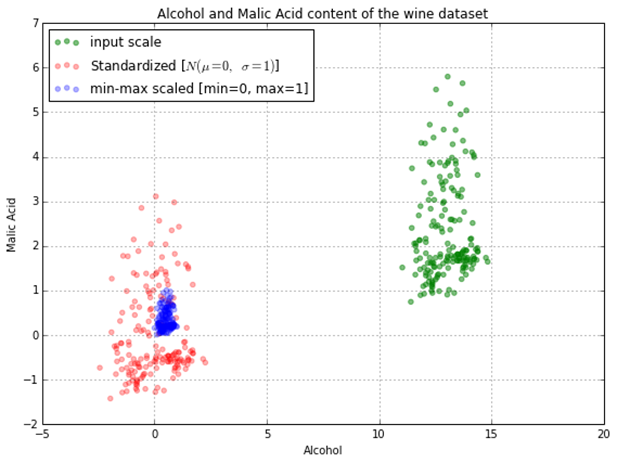
\includegraphics[scale=0.6]{scaling.png}
\end{figure}


\subsection{Standaryzacja}

\[x' = \frac{x - \bar{x}}{\sigma}\]

W ten sposób otrzymujemy zbiór ze średnią $\mu = 0$ oraz odchyleniem standardowym $\sigma = 1$.

\subsection{Normalizacja}

\[x' = \frac{x - \bar{x}}{\max(x) - \min(x)}\]

W ten sposób otrzymujemy wartości $x' \in [-1,1]$ ze średnią $\mu = 0$.

\subsection{Min-max}

\[x' = \frac{x - \min(x)}{\max(x) - \min(x)}\]

W ten sposób otrzymujemy wartości $x' \in [0,1]$.

\section{Skalowanie a trening}

Skalowanie zbioru danych ma też pozytywny wpływ na szybkość uczenia lub dokładność modelu w zależności od metody.

\subsection{Gradient decent}

\begin{figure}[H]
    \centering
    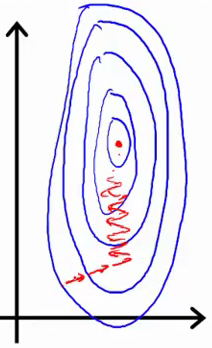
\includegraphics[scale=0.4]{no_scaling.png}
    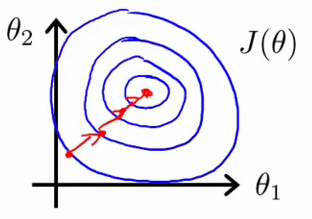
\includegraphics[scale=0.6]{yes_scaling.png}
\end{figure}

Jeśli dane są rozciągniete w jednym z wymiarów (ma duże odchylenie standardowe), gradient może długo skakać na drodze do optimum. Kiedy przeskalujemy te dane droga do rozwiązania optymalnego jest łatwiejsza.

\subsection{KNN}

\begin{figure}[H]
    \centering
    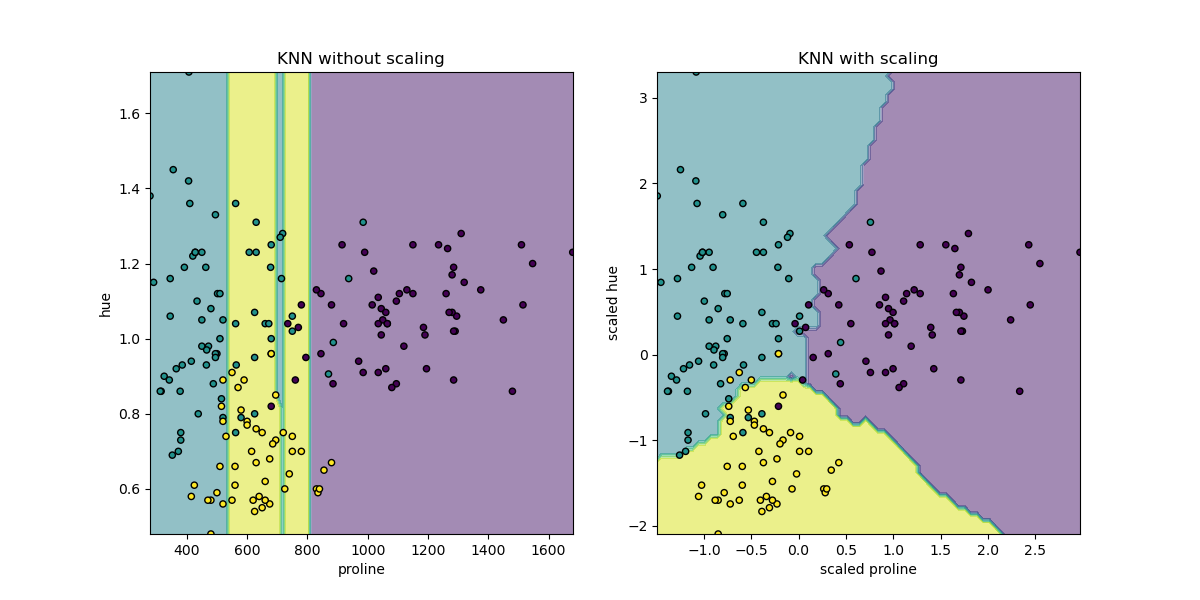
\includegraphics[scale=0.5]{knn.png}
\end{figure}

Jak widzimy dane oryginalne oraz przeskalowane prowadzą do powstania zupełnie różnych modeli.

\subsection{Modele oparte o drzewa}

W modelach opartych o drzewa wpływ sklaowania jest znikomy.

\end{document}